%! Author = sbbfti
%! Date = 10/06/2020
\section{Results and Discussion}\label{sec:results}

\subsection{Comfort DB overview}\label{subsec:comfort-db-overview}
While the \gls{db2} contains \var{entries_db_all}, only a total of \var{entries_db_used} entries met the inclusion criteria listed in the Methodology Section.
The distribution of the six input variables used to calculate the PMV indices is depicted in Figure~\ref{fig:dist_input_data}.

\begin{figure*}[htb!]
    \centering
    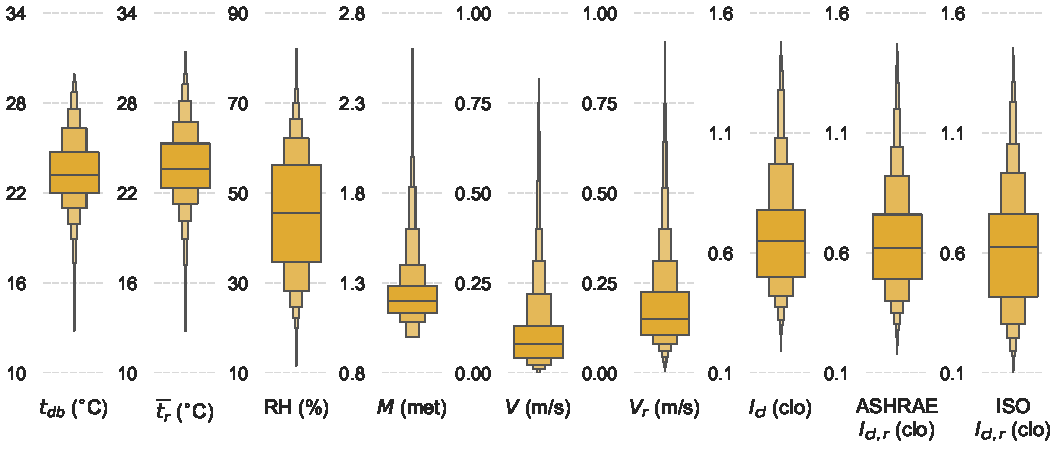
\includegraphics[width=\textwidth]{figures/dist_input_data}
    \caption{Distribution of the input variables used to calculate the \ac{pmv} values.
    The text in blue is showing the the 2.5th, 50th (median), and 97.5th percentiles.
    The data are shown using boxen-plots (letter-value plots).
    They depict the median as the centerline and each successive level outward contains half of the remaining data.}
    \label{fig:dist_input_data}
\end{figure*}

Figure~\ref{fig:dist_input_data} also depicts the 2.5th, 50th (median), and 97.5th percentiles for all the input variables.
We were not able to determine the accuracy of the \ac{pmv} formulations for inputs which were lower than the 2.5th and 97.5th percentiles, since we only had a limited number of datapoints beyond those limits.
Moreover, the distribution of these data was not uniform across the Standard's applicability ranges.
For example, only 2.5\% of the available dataset had a \ac{tdb} $\leq$ than \var{ta_95_perc_min}.
This can be explained by the fact that only few buildings across the globe have operate at \ac{tdb} lower than this value.
Which would be deemed to be unsatisfactory by a great number of occupants.
Consequently, we were not able to validate the accuracy of both formulations beyond these limits, despite the fact that both thermal comfort Standards applicability limits extend to \qty{10}{\celsius}.
This lack of data is particularly relevant for \ac{v}.
The \ac{pmv} and \gls{pmv-ce} only differ when the value of \ac{v} exceeds \qty{0.1}{\m\per\sec}, however, due to the fact that most of the entries in the \gls{db2} were collected in buildings with low air movement we could not reliably test the accuracy of the \ac{pmv} formulations for values of \ac{v} higher than \var{v_95_perc_max}.

Figure~\ref{fig:dist_other_data} shows the distribution of the age, height, weight, and running mean outdoor temperature grouped by sex.
Less than half (\num{23300}) of the total entries had information about the participant's sex.
Out of those data were almost equally distributed among male \qty{52}{\percent} and females.
Ages are not normally distributed, the same is true for the running mean outdoor temperature.
About half of the participants (\qty{52}{\percent}) were aged between \num{20} and \num{35} years old, and only \qty{2.5}{\percent} were older than 60.
This limits our analysis to healthy adults, and does not allow us to determine the accuracy of the \ac{pmv} model in predicting thermal sensation for children or older adults.
Approximately \qty{56}{\percent} of the running mean outdoor temperature values where between \qtyrange{10}{25}{\celsius}.
Men were significantly heavier and taller than females.
\begin{figure*}[htb!]
    \centering
    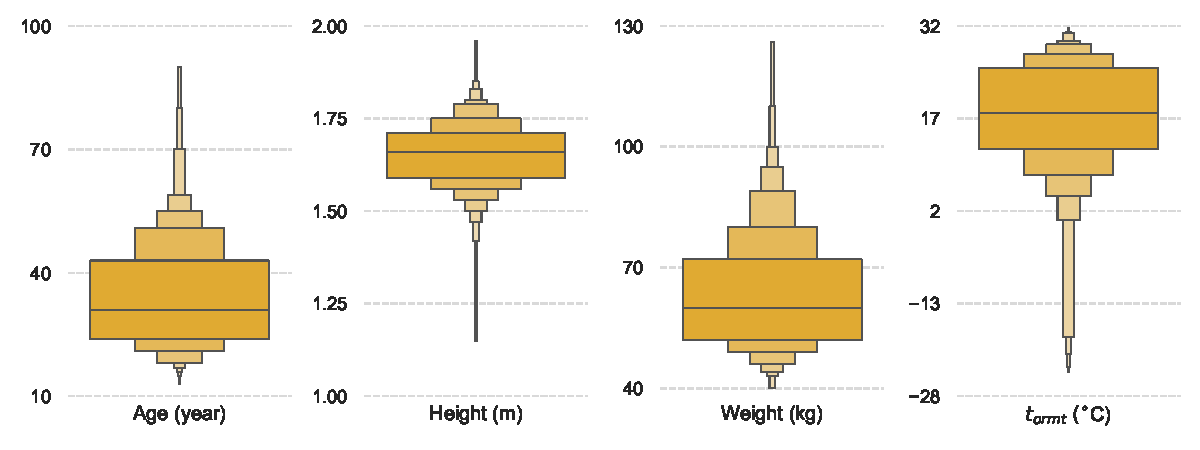
\includegraphics[width=\textwidth]{figures/dist_other_data}
    \caption{Distribution of age, height, weight, and running mean outdoor temperature.
    The data are grouped by sex.
    The text in blue is showing the the 2.5th, 50th (median), and 97.5th percentiles.}
    \label{fig:dist_other_data}
\end{figure*}
The percentage of \ac{tpv} grouped by each \ac{tsv} is shown on the left side of Figure~\ref{fig:bar_plot_tp_by_ts}.
Only \var{entries_with_tp} entries had information about both \ac{tsv} and \ac{tpv}.
Thus, on the right we show a bar chart depicting the distribution of all the \ac{tsv} votes, we have used in the analysis.
The \gls{db2} in respect to the \ac{tsv} is unbalanced.
Approximately \var{perc_tsv_neutral} of all the entries have a \ac{tsv} of `Neutral'.
While less than \var{perc_tsv_hot} of the total sample of participants reported to be either `Hot' or `Cold'.
\begin{figure*}[htb!]
    \centering
    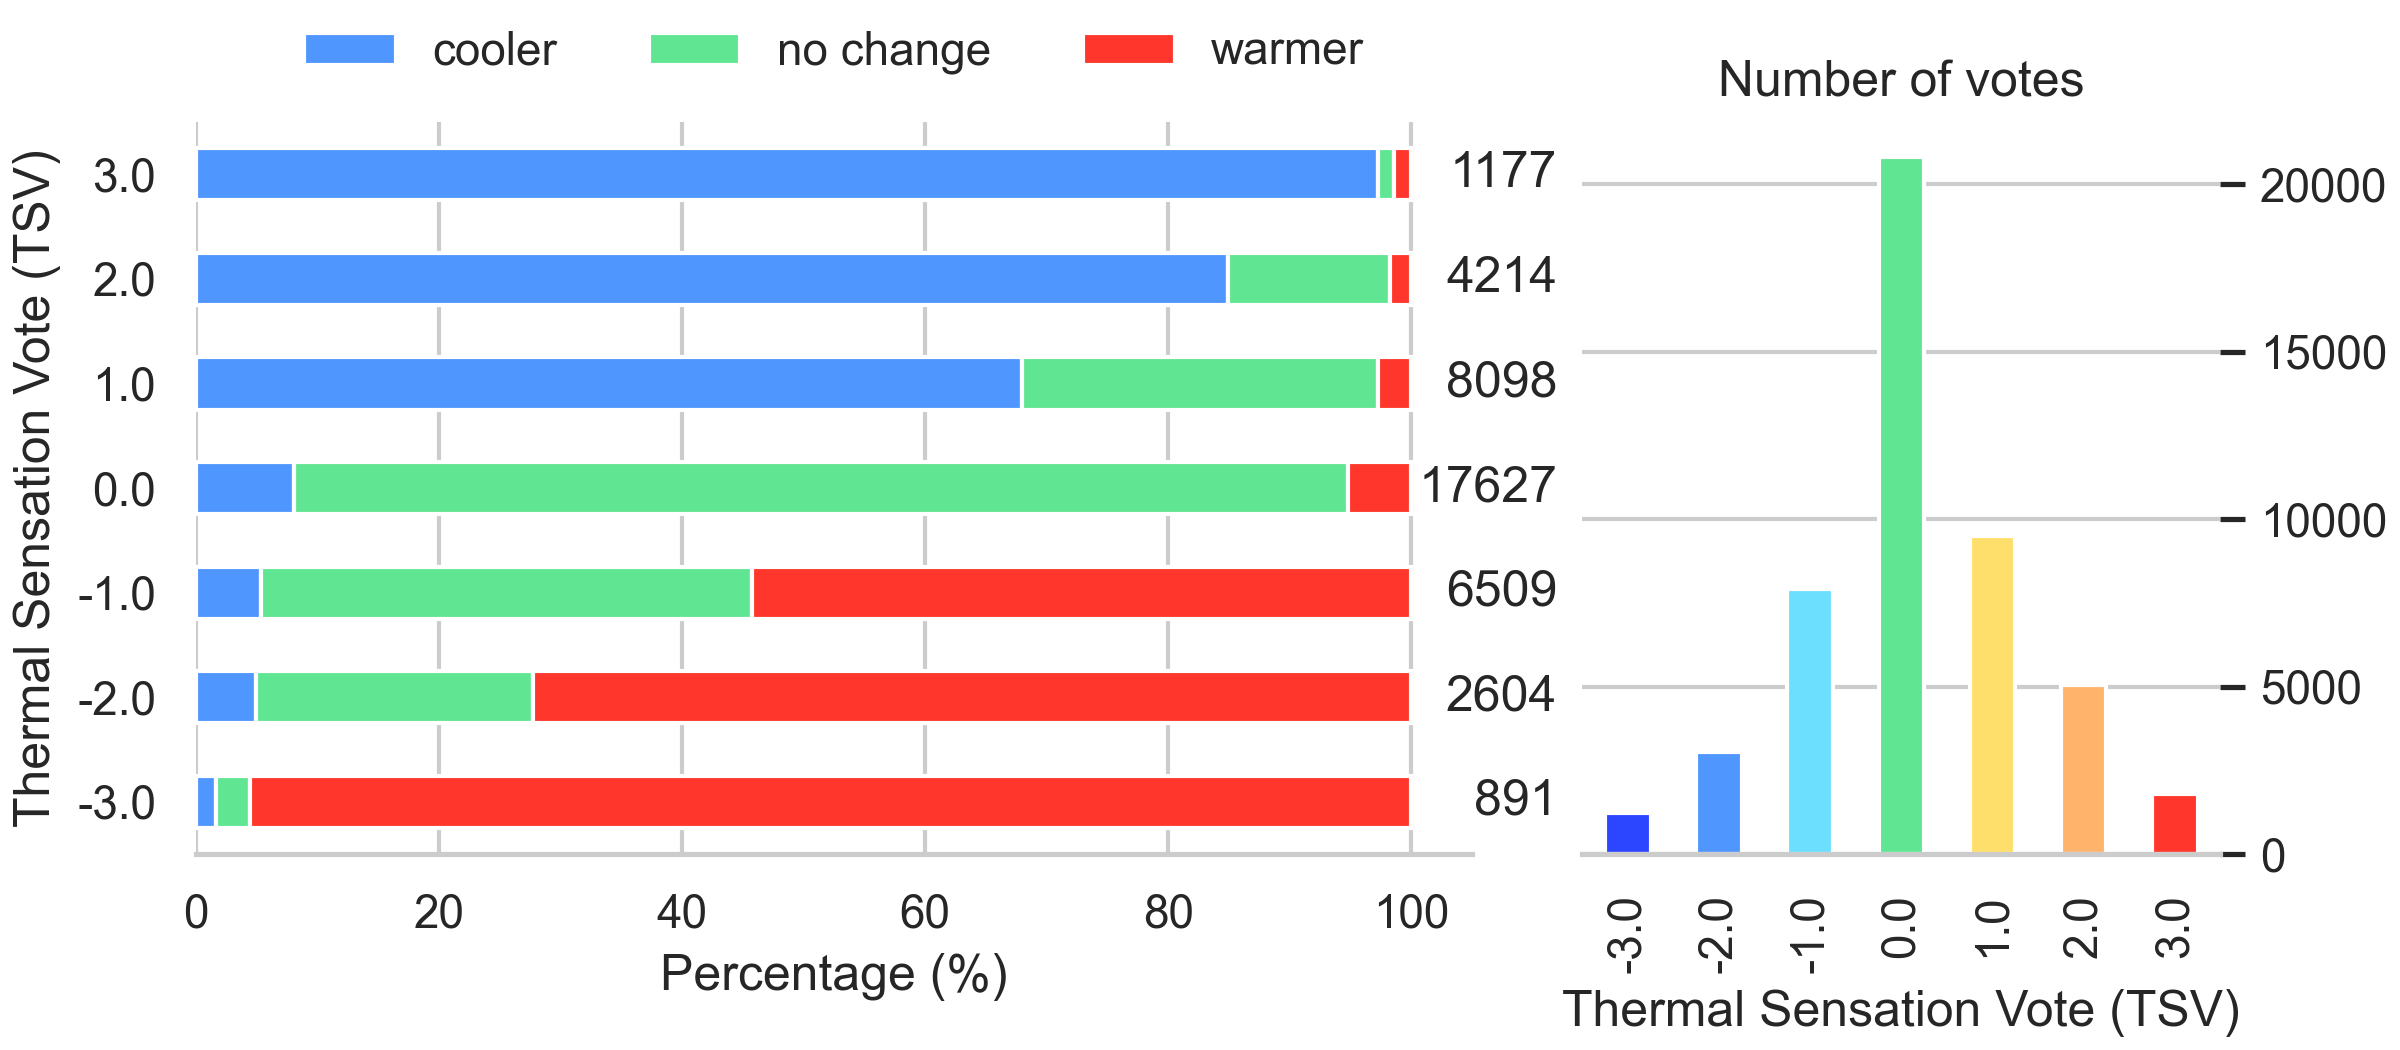
\includegraphics[width=\textwidth]{figures/bar_plot_tp_by_ts}
    \caption{The left Figure shows the percentage of \ac{tpv} for each thermal sensation vote.
    The numbers on the right side of each bar show the number of points for each \ac{tsv}.
    The right figure shows the total number of data points grouped by \ac{tsv}.
    Each bin in the Figure of the right has more data points than in the Figure on the left since information about the occupants \ac{tpv} were not always available.}
    \label{fig:bar_plot_tp_by_ts}
\end{figure*}
In thermal comfort research it is generally assumed that people who are `slightly warm' or `slightly cool' are thermally comfortable.
However, in the \gls{db2} more than \qty{50}{\percent} of participants who were either `slightly warm' or `slightly cool' wanted to be `cooler' or `warmer', respectively.
This finding challenges the above assumption.
This result suggests that the use of the thermal preference scale is better suited to determine how people perceive their thermal environment.
The \ac{tpv} clearly allows to determine whether participants would take action or not to modify their current thermal environment.
The \ac{tsv}, on the contrary, is ambiguous and does not allow to determine which actions should be taken to increase thermal comfort conditions for occupants.

\subsection{Comparison of PMV accuracy in predicting thermal sensation}\label{subsec:model-accuracy-comparison-in-predicting-thermal-sensation}
The \ac{pmv} was developed with the primary aim of predicting \ac{tsv}, consequently, in this Section we are reporting the prediction accuracy of different \ac{pmv} formulations.

\begin{figure*}[htb!]
    \centering
    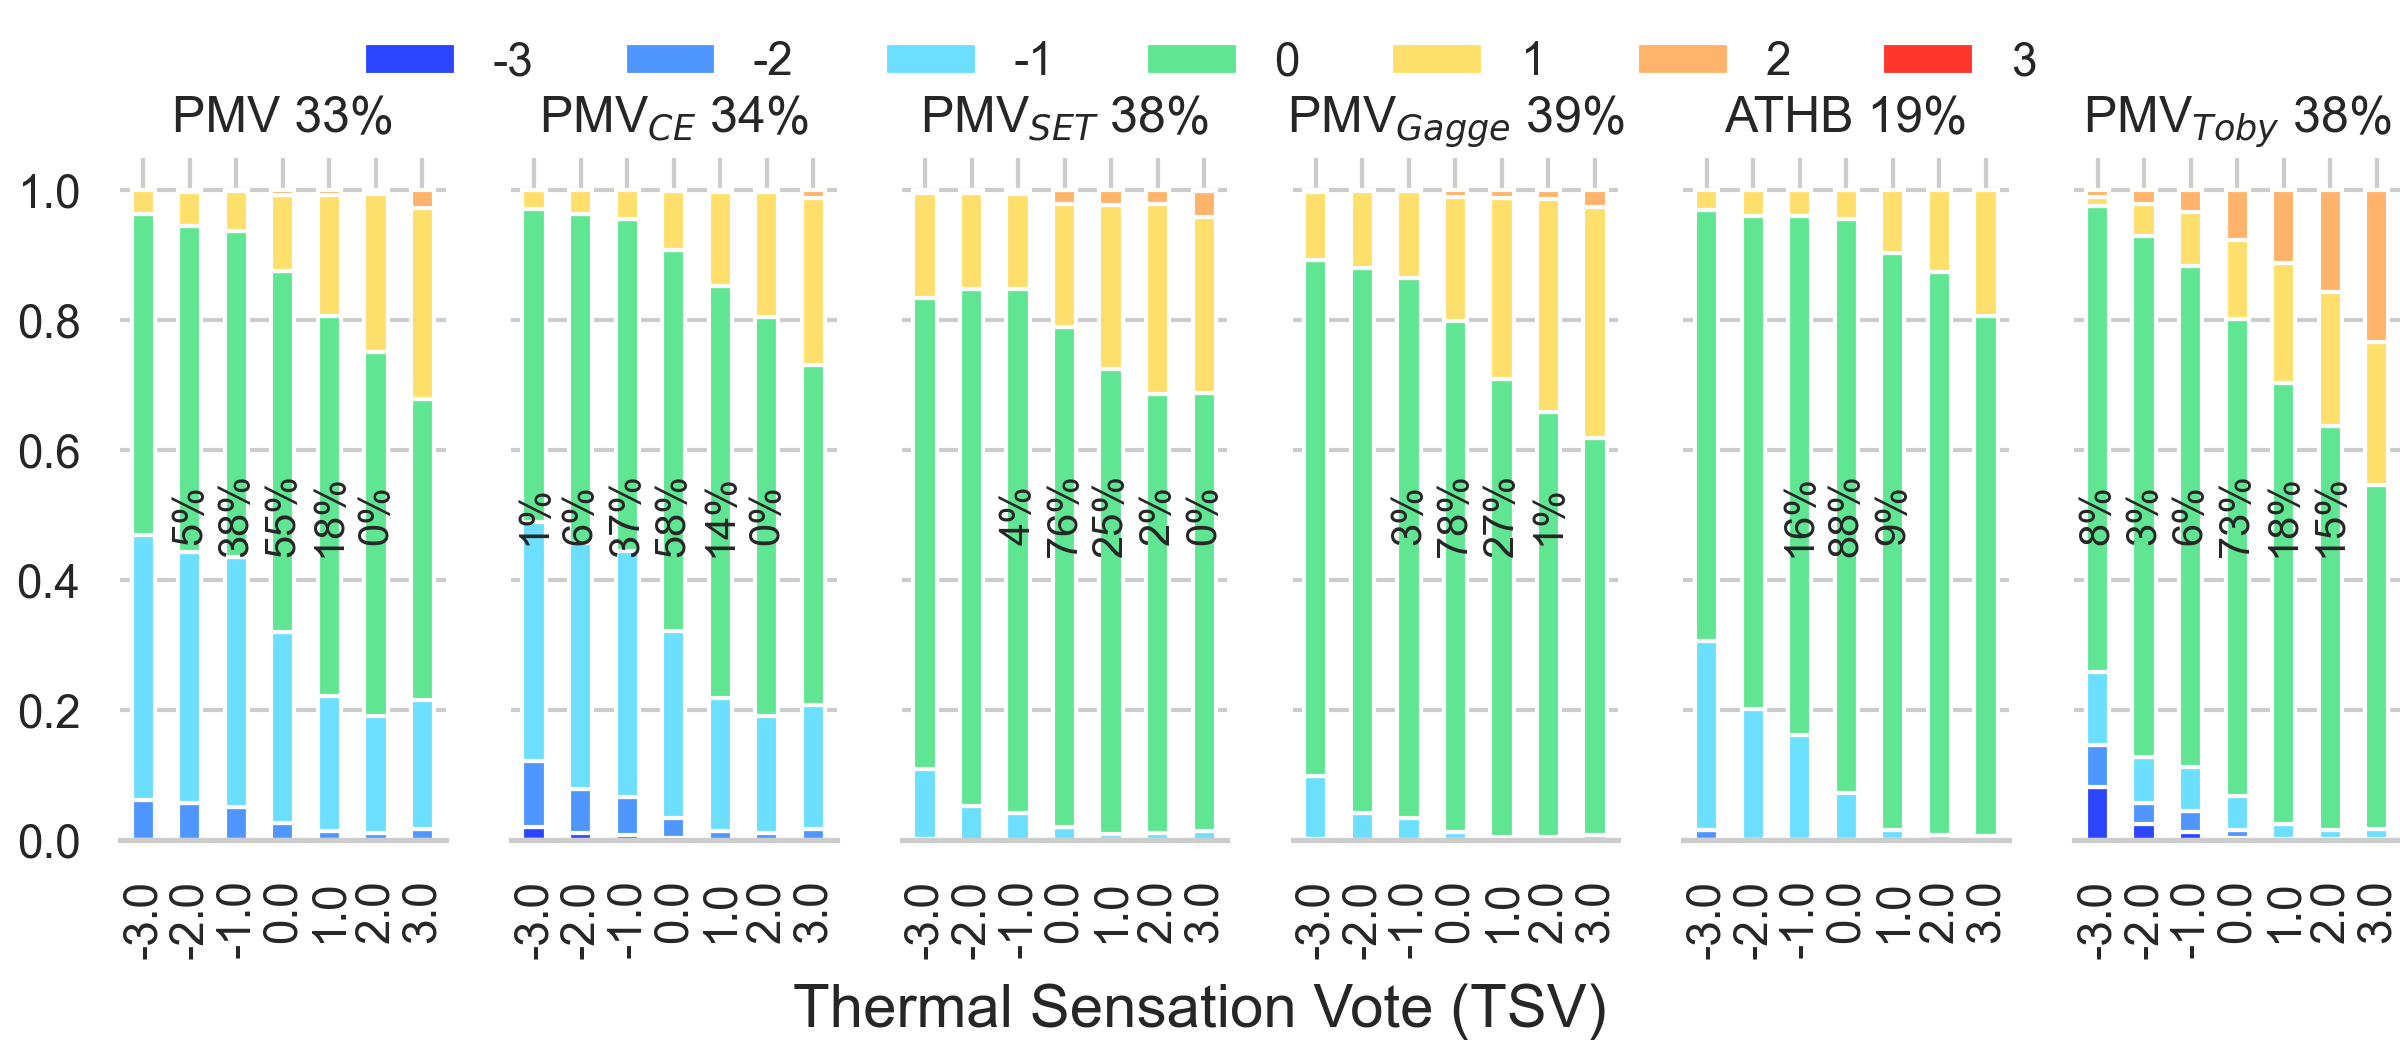
\includegraphics[width=\textwidth]{figures/bar_stacked_model_accuracy}
    \caption{}
    \label{fig:bar_stacked_model_accuracy}
\end{figure*}

Being \ac{tsv} the value reported by participants (i.e., ground truth) we grouped participants responses by \ac{tsv} and reported the simple accuracy of the different \ac{pmv} formulations in Figure~\ref{fig:bar_stacked_model_accuracy}.
In other words, all \ac{pmv} formulations underestimated the conditions at which participants are thermally dissatisfied with their environment.
The overall accuracy of the \gls{pmv-ce} and \ac{pmv} were \qty{34}{\percent} and \qty{33}{\percent}, respectively.
Being the classification problem unbalanced the simple accuracy is not an optimal metric to rate the model prediction accuracy since a default strategy of guessing the majority class would lead to a high overall model accuracy.
A model that would have predicted always `neutral' would have achieved an overall accuracy of \var{perc_tsv_neutral}, which is the number of participants who voted \ac{tsv}=0.
For this reason in Table~\ref{tab:f1} we report the F1-scores for all the models.
The F1-macro score which is free from label imbalance depicts that the accuracy of both models across all metrics is marginally better to random guessing (i.e., \qty{14.3}{\percent}).

\begin{table}[htb!]
    \centering
    \begin{tabular}{lccc}
\toprule
F1 score & PMV & PMV$_{CE}$ & Dataset \\
\midrule
 micro & 0.32 & 0.34 & \multirow{3}{*}{All data} \\
macro & 0.16 & 0.15 &  \\
weighted & 0.29 & 0.30 &  \\
\specialrule{.01em}{.05em}{.05em} micro & 0.32 & 0.35 & \multirow{3}{*}{\ac{vr} $\geq$ \qty{0.2}{\m\per\s}} \\
macro & 0.17 & 0.17 &  \\
weighted & 0.30 & 0.31 &  \\
\specialrule{.01em}{.05em}{.05em} micro & 0.30 & 0.31 & \multirow{3}{*}{\ac{vr} $\geq$ \qty{0.2}{\m\per\s} at three heights} \\
macro & 0.17 & 0.16 &  \\
weighted & 0.27 & 0.27 &  \\
\specialrule{.01em}{.05em}{.05em} micro & 0.43 & 0.45 & \multirow{3}{*}{$\lvert \textrm{PMV}\lvert \leq 1.5$ and $\lvert \textrm{TSV}\lvert \leq 1.5$} \\
macro & 0.23 & 0.22 &  \\
weighted & 0.42 & 0.43 &  \\
\bottomrule
\end{tabular}

    \caption{F1-score for the \ac{pmv} and \gls{pmv-ce} models.}
    \label{tab:f1}
\end{table}

Moreover, while the \gls{pmv-ce} was specifically developed to more accurately estimate latent and sensible heat losses from the skin to the environment.
Our results show that neither formulations can correctly classify participants who reported to be either `warm' or `hot' and the \gls{pmv-ce} is less accurate than the \ac{pmv} in predicting people who were `slightly warm'.
Both models had an accuracy lower than \qty{1}{\percent} when predicting wither `warm', `hot', or `cold'.
This value is significantly lower and worse than random guessing.

The low prediction accuracy of both models formulations coupled with the lack of data in the extremes of the applicability limits of the models, may suggest that the models applicability limits should be revisited and perhaps limited.
For example, Standards applicability limits could be limited to \qty{18}{\celsius} $\leq$ \ac{tdb} $\leq$ \qty{30}{\celsius} until more data are collected or the \ac{pmv} formulation is changed to better predict people who vote at the extremes of the thermal sensation scale.

Grouping the results into discrete categories introduces rounding errors since some participants reported \ac{tsv} on a continuous scale and the \ac{pmv} value is a continuous variables.
To compensate for this we plotted the \ac{pmv} values as a function of \ac{tsv} in Figure~\ref{fig:bubble_models_vs_tsv} and we plotted a lowess curve.
\begin{figure*}[htb!]
    \centering
    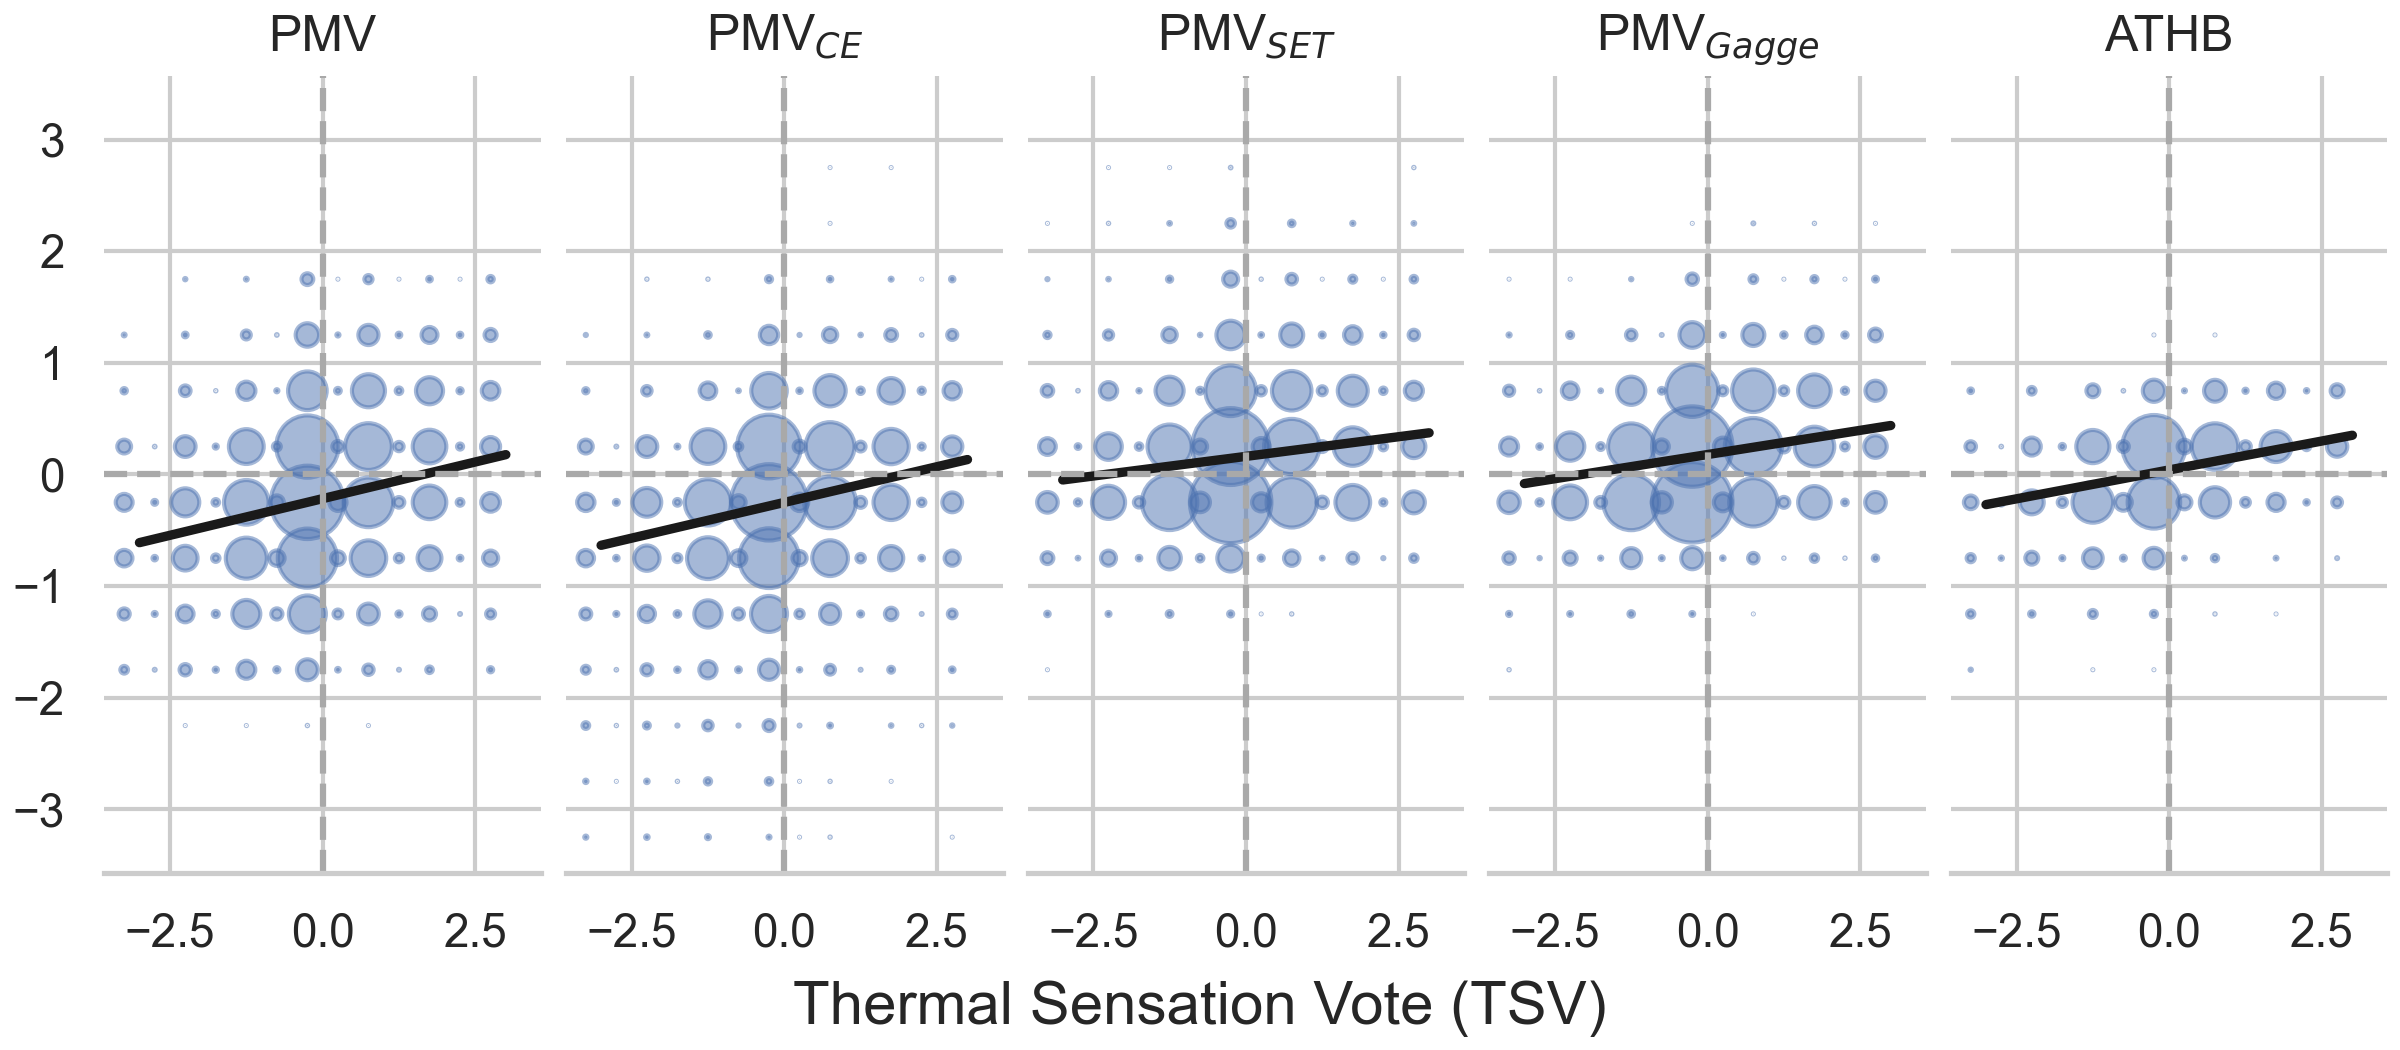
\includegraphics[width=\textwidth]{figures/bubble_models_vs_tsv}
    \caption{}
    \label{fig:bubble_models_vs_tsv}
\end{figure*}
The curve is calculated using the individual data and not the binned data.
We binned the data only to aid the visualization of a large dataset.
If the model is to accurately predict the thermal sensation of people, the regression line should pass through the origin of the cartesian plane and a slope of 1.
As depicted in Figure~\ref{fig:bar_stacked_model_accuracy}, while the regression line does not intercept is not zero, the intercepts for the \ac{pmv} is \qty{-0.23} and for the \gls{pmv-ce} is \qty{-0.24}.

\subsection{Model Bias}\label{sec:model-bias}
\subsubsection{Model Overall Bias}\label{subsec:model-overall-bias}
As previously mentioned in the Methodology section, the aim of the \ac{pmv} model is not to accurately predict each individual thermal response form participants.
The \ac{pmv} model was developed to predict the average thermal sensation of a large group of occupants sharing the same environment.
Consequently, while the above-mentioned analysis is informative in understanding the overall prediction error of the \ac{pmv} model it does compare individual \ac{tsv} to \ac{pmv}, hence it has some limitations, and it does not conclusively disprove the inefficacy of the \ac{pmv} model in predicting the average thermal sensation of a large group of occupants.

We calculated the overall bias of the model as previously done by \mycite{Humphreys2002} by subtracting the \ac{pmv} model prediction from the self-reported \ac{tsv}.
Results are presented in Figure~\ref{fig:hist_discrepancies}.
Overall both the \ac{pmv} and \gls{pmv-ce} models appear to be free from serius bias.
However, the \gls{pmv-ce} had a higher bias than the \ac{pmv} when using the full dataset, the summary statistics are shown in Figure~\ref{fig:hist_discrepancies}.
The median bias of the \ac{pmv} model reduced to \var{bias_median_pmv_0.2} from \var{bias_median_pmv_0} when we only included those datapoints with \ac{v} higher than \qty{0.2}{\m\per\s}.
While the opposite is true for the \gls{pmv-ce}, the median bias increased to \var{bias_median_pmv_ce_0.2} from \var{bias_median_pmv_ce_0}.

\begin{figure*}[htb!]
    \centering
    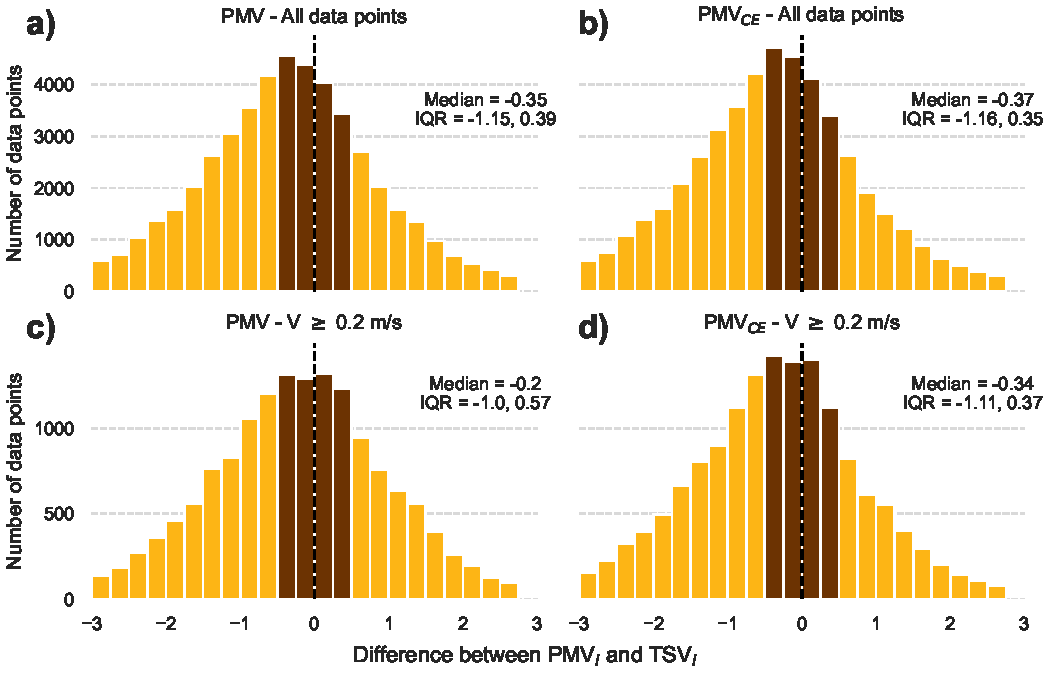
\includegraphics[width=\textwidth]{figures/hist_discrepancies}
    \caption{}
    \label{fig:hist_discrepancies}
\end{figure*}

\subsubsection{Model Bias as Function of Independent Variables, Thermal Sensation, Thermal Preference, and PMV}\label{subsec:model-bias-variable}
In the previous section we presented the overall bias of the two \ac{pmv} formulations.
We then went on determining how the bias varied as a function of \ac{tdb}, \ac{v}, \ac{met}, and \ac{clo}.
Figure~\ref{fig:dist_input_data} shows the results.
In each sub-figure we have binned the results into discrete intervals of equal width and the x-axis tick label is the center value of the bin interval. %and the width of the violin plot is linearly proportional to the number of points in that specific bin.
In each sub-figure, we kept data only above and below the 2.5th and 97.5th percentiles.
\begin{figure*}[htb!]
    \centering
    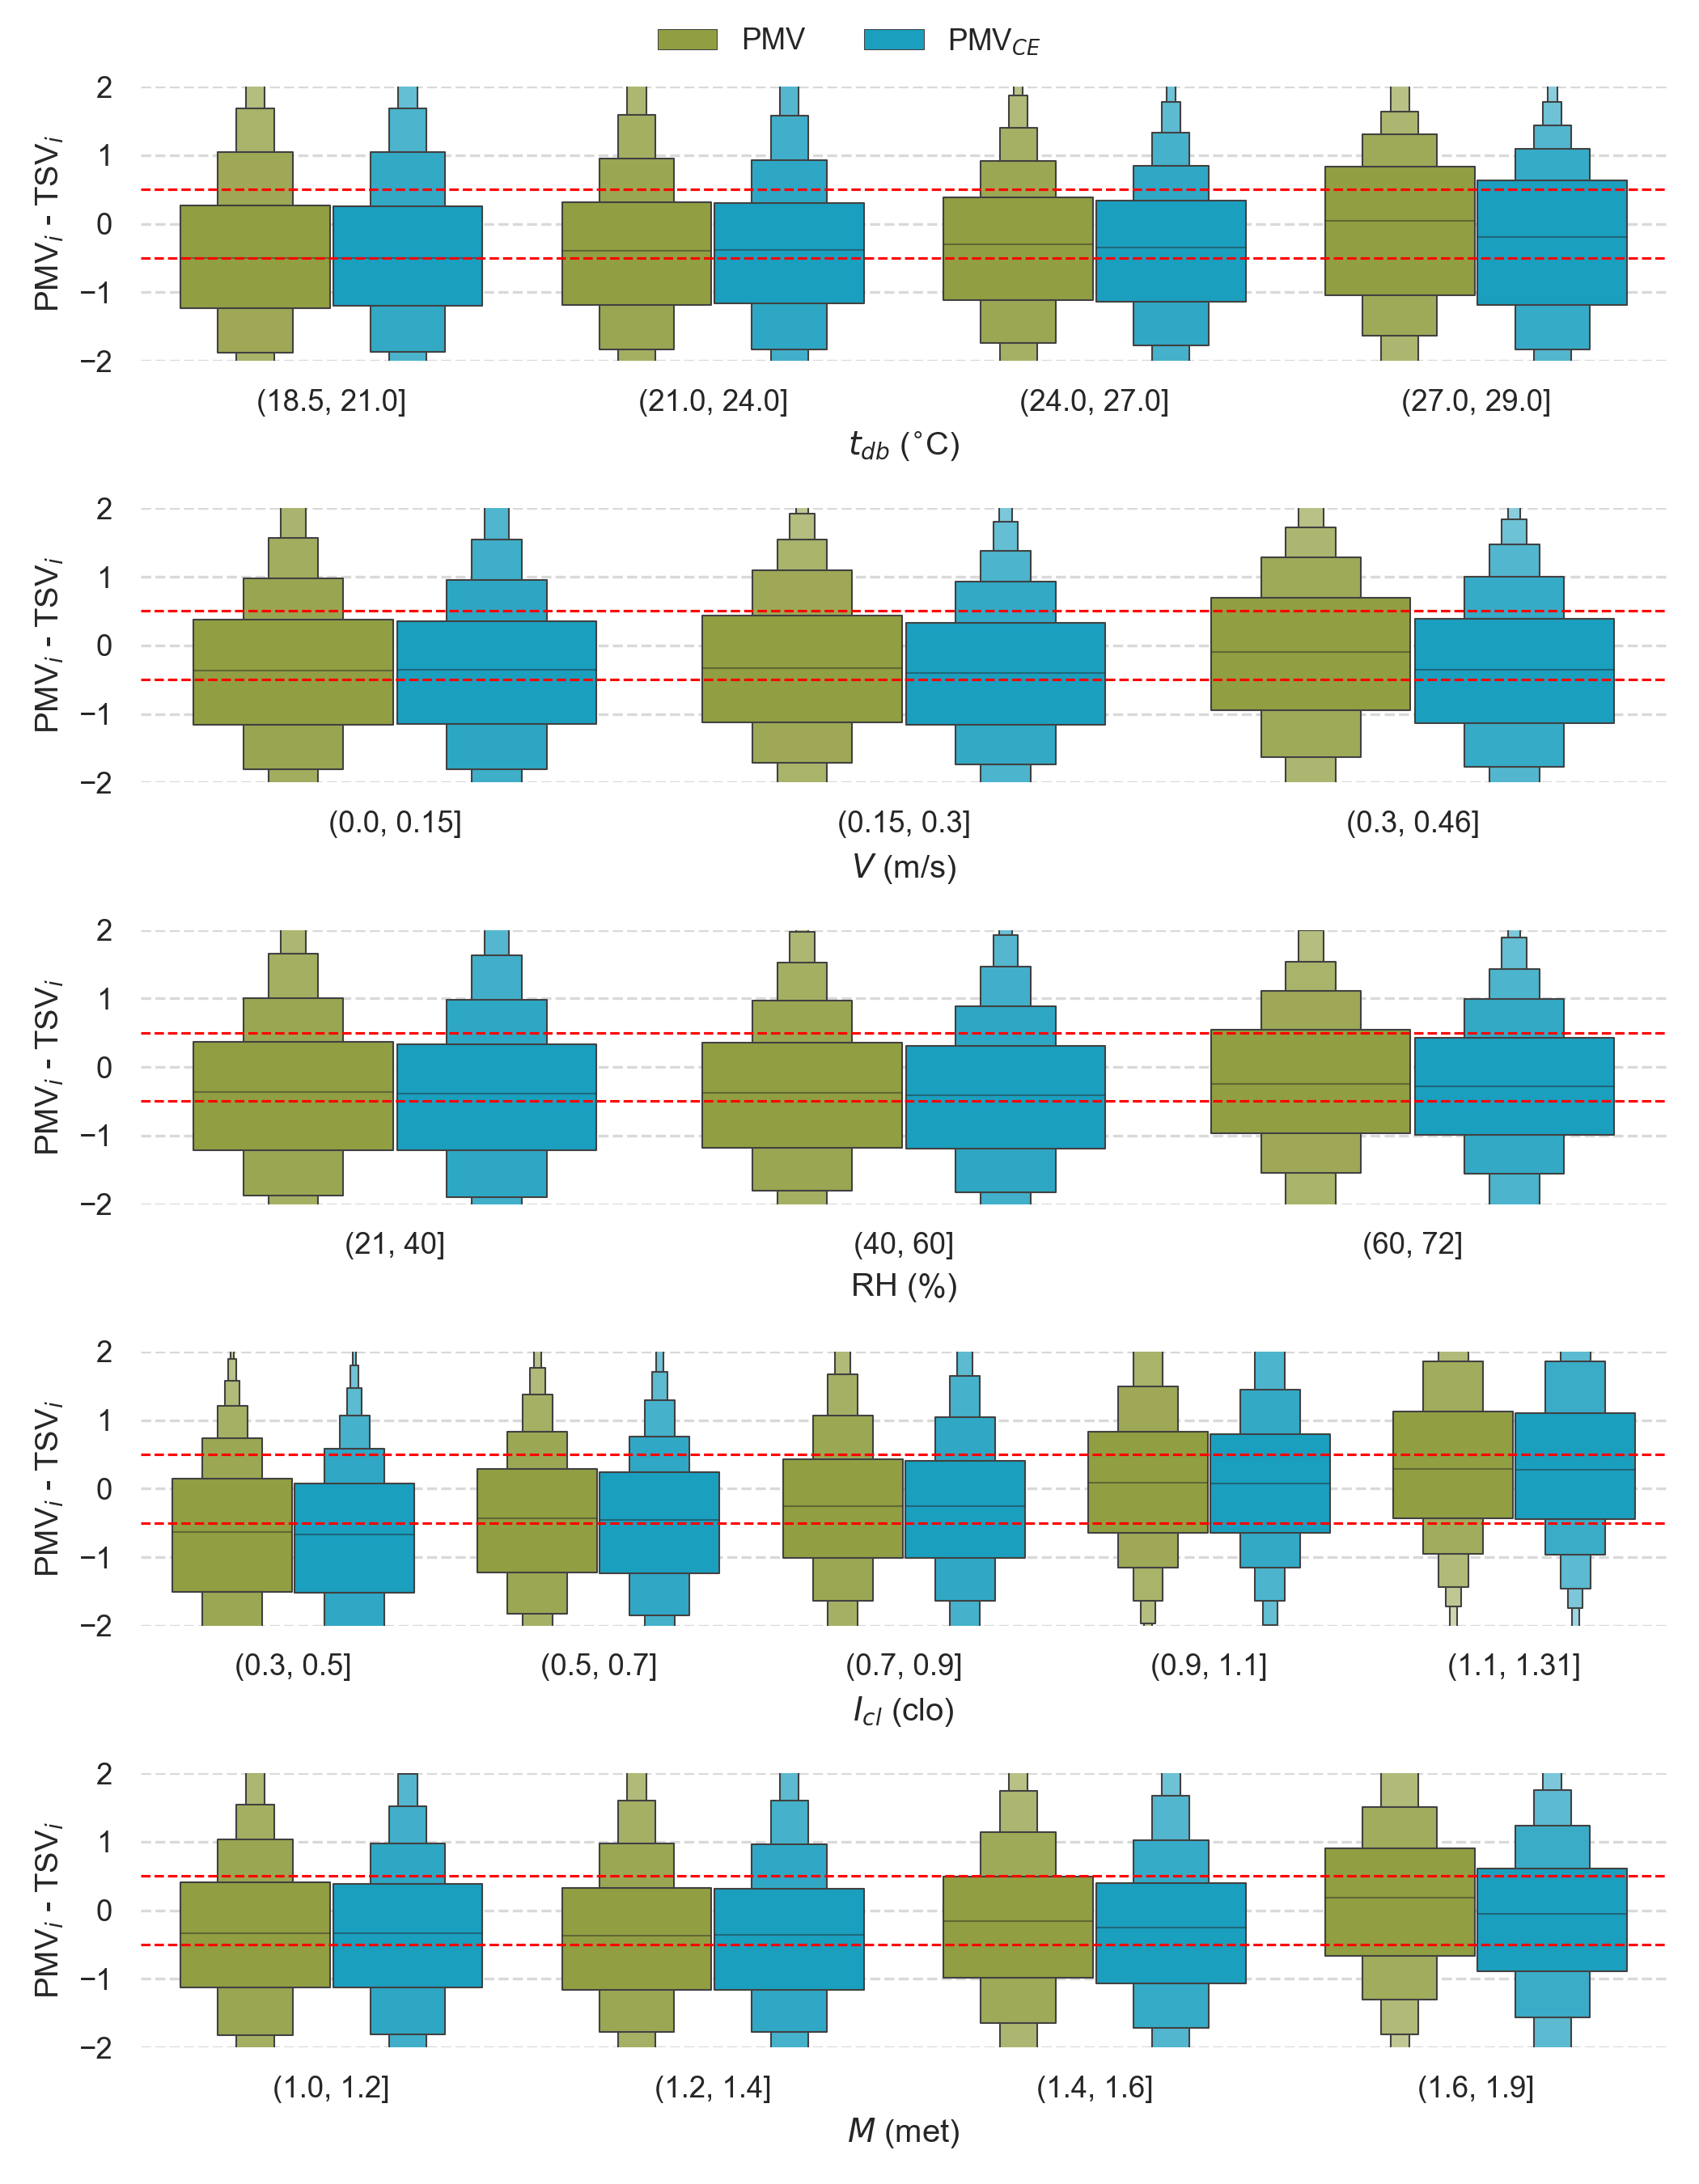
\includegraphics[width=\textwidth]{figures/bias_models}
    \caption{}
    \label{fig:bias_models}
\end{figure*}
The results depict that across the four input variables the use of the \gls{pmv-ce} model did not improve the bias of the model.
On the contrary, the bias of the \gls{pmv-ce} diverged more from 0 as the value of \ac{v} increased.
This outcome is particularly negative since the \gls{pmv-ce} was specifically developed to be more accurate than the \ac{pmv} at high airspeed.
These results are in agreement with those presented in the previous section.

\subsection{Comparison between the \ac{pmv} formulations wih the two-node model}\label{subsec:comparison-between-the-ac{pmv}-formulations-wih-the-two-node-model}
We then finally compared how the results of the \ac{pmv} and \gls{pmv-ce} compared with the results of the two-node model.
Figure~\ref{fig:pmv_two_node_comparison} was generated by calculating the \ac{pmv} using a combination of 5000 randomly generated sets inputs and using these to calculate the \ac{pmv} and \gls{pmv-ce} (y-axis), and the respective \gls{pmvg} value (x-axis).
The Figure also shows the locally weighted linear regression (LOWESS) curve.
The results of the \ac{pmv} model had a higher agreement with the results of the two-node model, in particularly for \gls{pmvg} $\geq$ \qty{0.5}{\m\per\s}.
Depicting the failure of the \gls{pmv-ce} model in achieving a greater achievement with the two-node model, despite using it in the backend to calculate the cooling effect.
\begin{figure*}[htb!]
    \centering
    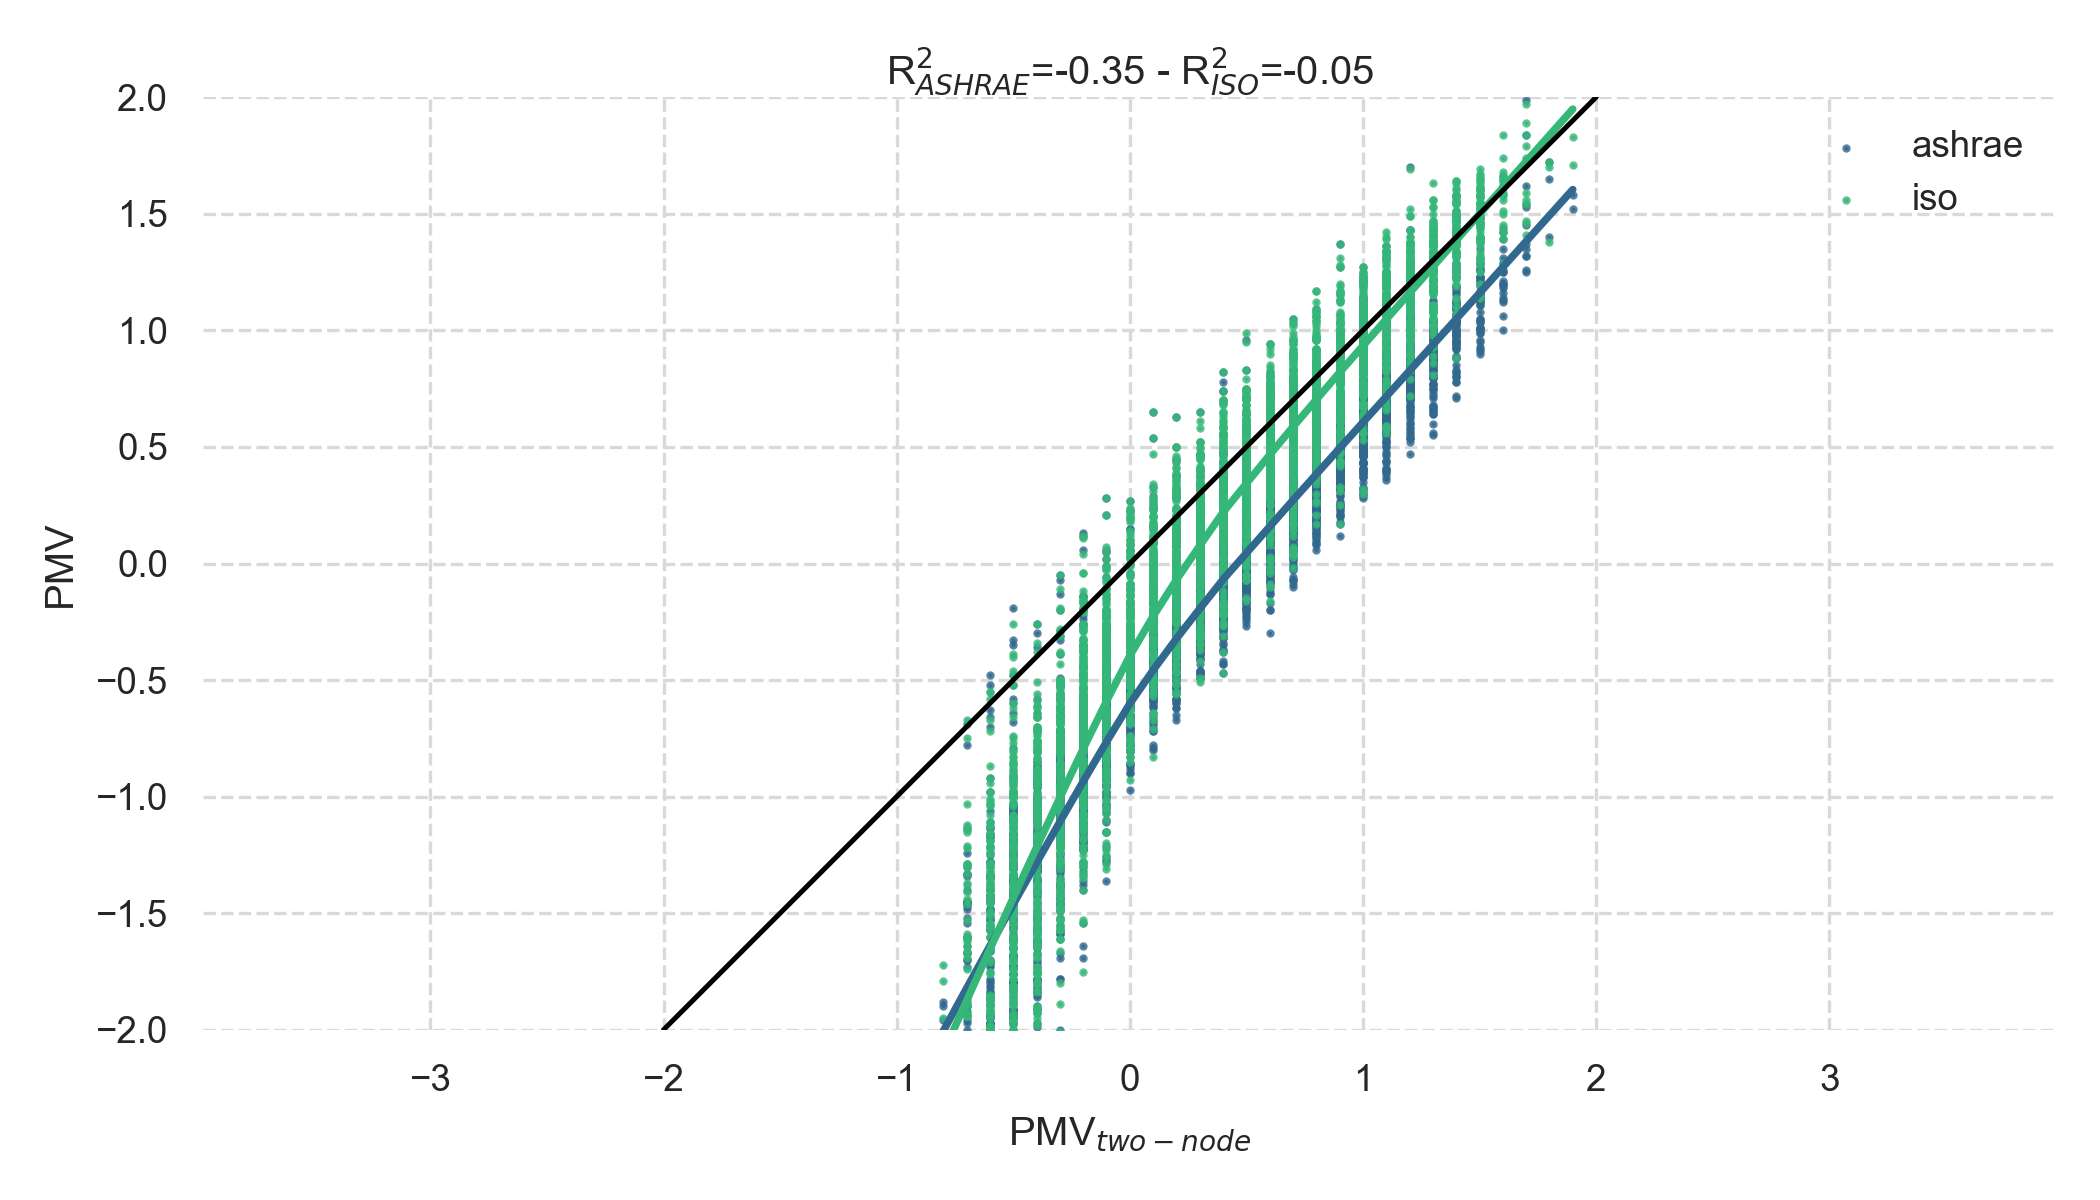
\includegraphics[width=\textwidth]{figures/pmv_two_node_comparison}
    \caption{}
    \label{fig:pmv_two_node_comparison}
\end{figure*}

\subsection{Sources of Error}\label{sec:sources-of-error}
While the scope of this manuscript is solely to compare the two \ac{pmv} formulations and determine which of the two is more accurate and should be used in thermal comfort standards.
In this section we are trying to identify some of the main reasons of why we observed in the predictive accuracy of the \ac{pmv} and \gls{pmv-ce} models when compared against the \ac{tsv} available in the \gls{db2}.

\paragraph{Lack of Data}
As previously mentioned several times the \ac{pmv} model aim to predict the average thermal sensation of a large group of occupants sharing the same environment.
First, the term `large' is vague and it leads to confusion since it is not clear what is the minimum number of people required, is it 2, 5, 10, or more?
Secondly, the data contained in the \gls{db2} do not contain information on where and when the thermal sensation votes where recorded and consequently we could not appropriately validate the accuracy of the model since in most of the analysis we ended up comparing single \ac{tsv} with the \ac{pmv} model output.
The only exception to this is when we assessed the overall model bias.

\paragraph{Heat Balance Equation and Calculation of the PMV value}
 The \ac{pmv} model uses simplified heat balance equations to estimate the heat loss and gains from the human body to its surrounding environment.
This in itself is a possible source of error since the model consider the human body to be a cilinder with constant width all uniformly covered with clothing were the heat is all generated in its core.
This is great simplification since it ignores the fact that different parts of the body may not be covered by clothing, the metabolic heat generation is not uniform, it ignores vasoconstriction and vasodilation, and most importantly it fundamentally assumes that the human body is never in thermal neutrality.
This is clearly not the case, since the human body in most conditions observed indoors in commercial buildings is capable of maintaining a constant core temperature.
The \ac{pmv} model then maps the heat loss or gains, which are a proxi to the thermal stress that the human body has to undergone to maintain a constant internal temperature to a \ac{pmv} value which should represent a \ac{tsv} vote.
Fanger created this equation based on a few experimental data collected in a laboratory, and despite the growing body of literature this equation was never updated.
Moreover, the heat losses and gains are mapped equally to a thermal sensation vote, disregarding that the human body does not have the same ability to compensate for warm and cold conditions.
It is, therefore, not surprising to observe that the \ac{pmv} model has an acceptable accuracy in determining when people are `neutral` which is equivalent to a \ac{pmv} of 0 and the body is dissipating all the internal metabolic heat production trough conduction, convection, or radiation.
On the other hand the model is not capble of identifying people at either extremes of the \ac{tsv} scale.
These people most likely were exposed to compensable conditions, which in other words means that their core temperature remain constant.
However, their body either used vasocontriction to compensate for the heat losses, or a combination of vasodilation and sweating to compensate for heat gains.
More research is need to determine whether the inacuracy of the model is related to either or a combination of the following factors: i) assuming that the heat lossess/gains estimated by the \ac{pmv} should represent the thermal stress the body has to udertake to compensate for unsatisfactory thermal comfort conditions is not correct;
ii) the relationship between the heat lossess/gains and thermal stress is different from the one assumed by Fanger;
iii) heat losses and gains correlation to thermal stress is not not the same and two equations should be used;
iv) the mapping of the \ac{pmv} to the \ac{tsv} uses a different anchor from what participants use in reporting thermal sensation.
For example, while the \ac{pmv} model may assume that a score of 3 signify the change between a compensable set of conditions to an uncompensable one, e.g., their skin wettedness reaches the max value ($w_{max}$).
Participants in commercial buildings may, on the contrary, deem the environment to by `Hot' as soon as they start sweating, or in technical words their skin wettedness crosses a critical threshold which is only a fraction of $w_{max}$.
It is likely that a combination of the above mentioned factors play a role, but only the latter has gained more momentum in the literature which led to development of several \ac{pmv} where the final value was multipled by a constant generally lower than one.
While few of these indices tried to change the intercept.

\paragraph{Measurement Errors}
While all the data contained in the \gls{db2} have been published in peer-reviewed manuscript measurements errors are inevitably present in the dataset.
This is due to the accuracy of the instrumentation used, the placement of the instrumentation, and the estimation of clothing, and activity using reference tables.
In an ideal scenario, errors may be random and would cancel out and not affect the overall bias of the model but only the standard deviation of the error, however, this may not always be the case, for example if a researchers often underestimated the clothing insulation of participants or their activity levels.

\paragraph{Thermal Sensation Scale}
One minor but not negligible source of error is the use of a discrete scale to assess thermal sensation.
Most of the \ac{tsv} in the \gls{db2} were collected using a discrete scale while the \ac{pmv} output is continuous.
For example, even if the model was 100~\% accurate and the estimated \ac{pmv} values was \num{2.5} the person could only report to be `warm (+2)' or `hot (+3)'.
% talk also about the research we published with Marcel and how participants perceive the thermal sensation scale

\paragraph{Thermal Sensation Scale}
Errors are also caused by the fact that the \ac{pmv} model is an approximation of a highly complex system (the human body and mind) which interacts with the surrounding environment.
Fanger could not, therefore, include all the factors that contribute to the comfort vote and some of them have been omitted.
Finally, it should be noted that the \ac{pmv} model has been developed considering based on the assumption of steady-state heat transfer, however, this never precisely occurs since the human thermo regulatory system is always actively engaged to ensure a stable core temperature.
However, as \mycite{Humphreys2002} note, these approximations and errors present in the \ac{pmv} model, if the model is accurate, should combine to produce a quasi-random error in the prediction.
This would increase the standard deviation of the delta between the \ac{tsv} and \ac{pmv}, but if the model is sound, they should produce a negligible bias~\cite{Humphreys2002}.
On the other hand, if the model is neither accurate nor representative of the real system a significant bias will arise.